% ==============================================================================
% PHẦN A: TÌM HIỂU HỆ QUẢN TRỊ CƠ SỞ DỮ LIỆU PHÂN TÁN TiDB
% (Chiếm 50% nội dung báo cáo theo đúng định hướng của giảng viên)
% ==============================================================================

\phanbaocao{PHẦN A}{TÌM HIỂU HỆ QUẢN TRỊ CƠ SỞ DỮ LIỆU PHÂN TÁN TiDB\\--- TỪ ĐẶC TRƯNG DỮ LIỆU ĐẾN KIẾN TRÚC VÀ CÀI ĐẶT}

\section{Xuất phát từ Đặc trưng Dữ liệu: Phân loại Dữ liệu và Lý do chọn TiDB (NewSQL)}
\label{sec:phan_a_dac_trung_du_lieu}

\subsection{Phân loại các dạng dữ liệu và bài toán thực tế}

Trong bối cảnh bùng nổ dữ liệu hiện đại, việc lựa chọn hệ quản trị cơ sở dữ liệu (DBMS) phù hợp phải bắt đầu từ việc thấu hiểu bản chất và đặc trưng của mô hình dữ liệu cần lưu trữ, cũng như các ràng buộc khắt khe về mặt nghiệp vụ giao dịch. Không tồn tại một hệ quản trị vạn năng (\textit{One Size Fits All}) giải quyết tối ưu cho mọi loại hình dữ liệu. Bảng~\ref{tab:so_sanh_he_quan_tri} tổng hợp phân loại bốn nhóm dữ liệu phổ biến, các hệ quản trị tiêu biểu và giới hạn cốt lõi của chúng khi đối mặt với bài toán giao dịch quy mô lớn.

\begin{table}[H]
\centering
\caption{Đối chiếu các dạng dữ liệu, hệ quản trị tiêu biểu và hạn chế khi xử lý quy mô lớn}
\label{tab:so_sanh_he_quan_tri}
\bangfont
\begin{tabularx}{\linewidth}{@{}>{\raggedright\arraybackslash}p{3.8cm}>{\raggedright\arraybackslash}p{2.6cm}Y@{}}
\toprule
\textbf{Dạng dữ liệu \& Bài toán} & \textbf{Hệ quản trị tiêu biểu} & \textbf{Hạn chế khi áp dụng vào Giao dịch Quy mô lớn (Massive OLTP \& HTAP)}\\
\midrule
\textbf{Dữ liệu Quan hệ truyền thống} (Vừa và nhỏ, lược đồ cố định, toàn vẹn tham chiếu) & MySQL (InnoDB), PostgreSQL & Kiến trúc nguyên khối (\textit{Monolithic}) gắn chặt Tầng Tính toán (Compute) và Tầng Lưu trữ (Storage) trên một máy chủ vật lý. Khi bảng vượt ngưỡng 50--100 triệu dòng (như case study bảng \code{activities} 1,47 tỷ dòng của Pipedrive), MySQL chịu hiện tượng nghẽn I/O đĩa, cạn kiệt Buffer Pool, nghẽn khóa khi thực thi câu lệnh DDL (\code{ALTER TABLE}) và nguy cơ sập toàn bộ dịch vụ nếu máy chủ đơn lẻ gặp sự cố (\textit{Single Point of Failure - SPOF}).\\
\midrule
\textbf{Dữ liệu Cột rộng / Chuỗi thời gian} (Wide-Column / Time-Series) & Apache Cassandra, HBase & Tối ưu cho thao tác ghi tuần tự cực nhanh và mở rộng ngang tuyến tính, tuy nhiên phải hy sinh tính chất giao dịch ACID đa dòng (\textit{Multi-row ACID}) và hoàn toàn không hỗ trợ câu lệnh \code{JOIN} phức tạp hay ngôn ngữ SQL quan hệ chuẩn.\\
\midrule
\textbf{Dữ liệu Tìm kiếm văn bản \& Đồ thị} (Full-Text Search / Graph) & Elasticsearch, Neo4j & Chuyên biệt cho truy vấn đảo nghịch (\textit{Inverted Index}) hoặc duyệt đồ thị đỉnh-cạnh (\textit{Graph Traversal}). Không được thiết kế làm hệ thống ghi nhận giao dịch cốt lõi (\textit{System of Record}) do chi phí duy trì tính nhất quán tuyệt đối là rất lớn.\\
\midrule
\textbf{Dữ liệu Giao dịch Quy mô lớn đòi hỏi ACID + Mở rộng ngang + Phân tích thời gian thực} & \textbf{TiDB (Distributed NewSQL)} & \textbf{Lý do chọn TiDB:} Giữ nguyên vẹn mô hình Bảng quan hệ (Relational Schema, ràng buộc toàn vẹn, khóa chính, chỉ mục phụ, giao dịch ACID đầy đủ) và tương thích hoàn toàn giao thức MySQL, nhưng bên dưới được chia nhỏ tự động thành các cặp Key-Value phân tán đa máy chủ. TiDB giải quyết triệt để nút thắt cổ chai về lưu trữ và chịu tải của RDBMS truyền thống.\\
\bottomrule
\end{tabularx}
\end{table}

\subsection{Bài toán đặt ra và lý do lựa chọn hệ quản trị NewSQL TiDB}

Từ bảng so sánh trên, bài toán trọng tâm đặt ra là: \textit{Làm thế nào để một hệ thống vừa giữ được tính tiện dụng và an toàn tuyệt đối của chuẩn SQL/ACID (vốn là chuẩn mực sống còn trong các hệ thống ngân hàng, thương mại điện tử, quản lý đơn hàng), vừa sở hữu năng lực mở rộng ngang vô hạn (Elastic Horizontal Scalability) và tính sẵn sàng cao (High Availability) của thế giới NoSQL?}

Đây chính là tiền đề ra đời của dòng hệ quản trị \textbf{NewSQL}, đại diện tiêu biểu là \textbf{TiDB} (được phát triển bởi PingCAP, lấy cảm hứng từ kiến trúc Google Spanner và F1). TiDB được lựa chọn làm hệ quản trị nghiên cứu chính trong đề tài này nhờ 4 phẩm chất cốt lõi:
\begin{enumerate}
  \item \textbf{Khả năng mở rộng ngang trong suốt (Transparent Horizontal Scalability):} Người dùng và ứng dụng nhìn vào cụm TiDB như một máy chủ MySQL duy nhất. Khi dung lượng hoặc số lượng kết nối tăng vọt, người quản trị chỉ cần bổ sung thêm các máy chủ vật lý mà không phải sửa đổi mã nguồn ứng dụng hay can thiệp chia bảng thủ công (\textit{Application-level Sharding}).
  \item \textbf{Tính sẵn sàng cao và Không mất dữ liệu (High Availability \& Zero Data Loss):} Triển khai thuật toán đồng thuận Multi-Raft, đảm bảo $RPO = 0$ (Recovery Point Objective) và $RTO \le 10\text{s}$ (Recovery Time Objective) ngay cả khi một phần ba số máy chủ lưu trữ bị phá hủy đột ngột.
  \item \textbf{Hỗ trợ xử lý lai giao dịch và phân tích (Hybrid Transactional/Analytical Processing - HTAP):} Cho phép truy vấn báo cáo phân tích trực tiếp trên dữ liệu giao dịch tươi mới nhất mà không làm ảnh hưởng đến độ trễ của các luồng ghi OLTP.
\end{enumerate}

% ==============================================================================
\section{Các Đặc trưng Kiến trúc Cốt lõi làm nên Sức mạnh của TiDB}
\label{sec:phan_a_kien_truc_tidb}

\subsection{Đặc trưng 1: Tách biệt hoàn toàn Tầng Tính toán (Compute) và Tầng Lưu trữ (Storage)}

Khác biệt căn bản nhất giữa kiến trúc phân tán của TiDB và kiến trúc nguyên khối của MySQL InnoDB nằm ở việc tách rời hoàn toàn giữa Tầng Tính toán (\textit{Compute Layer}) và Tầng Lưu trữ (\textit{Storage Layer}) thành hai cụm phần mềm hoạt động độc lập (Hình~\ref{fig:kientruc_tongthe_tidb}):

\begin{figure}[H]
\centering
\IfFileExists{figures/tidb_architecture.png}{
  \includegraphics[width=0.88\textwidth]{figures/tidb_architecture.png}
}{
  \begin{tikzpicture}[
    node distance=1.2cm,
    box/.style={draw=codeblue, thick, fill=blue!5, rounded corners, align=center, minimum width=3.2cm, minimum height=1cm, font=\small},
    storage/.style={draw=codegreen, thick, fill=green!5, rounded corners, align=center, minimum width=2.8cm, minimum height=1cm, font=\small},
    pdbox/.style={draw=codepurple, thick, fill=purple!5, rounded corners, align=center, minimum width=3.8cm, minimum height=1.1cm, font=\small}
  ]
    \node[pdbox] (pd) {Placement Driver (PD Cluster)\\Bộ não điều phối \& Timestamp Oracle (TSO)};
    \node[box, below left=1.2cm and 0.5cm of pd] (tidb1) {TiDB Server 1\\(Stateless SQL)};
    \node[box, below right=1.2cm and 0.5cm of pd] (tidb2) {TiDB Server 2\\(Stateless SQL)};
    \node[storage, below=1.4cm of tidb1] (tikv1) {TiKV Node 1\\(RocksDB / Raft)};
    \node[storage, below=1.4cm of pd] (tikv2) {TiKV Node 2\\(RocksDB / Raft)};
    \node[storage, below=1.4cm of tidb2] (tikv3) {TiKV Node 3\\(RocksDB / Raft)};

    \draw[<->, thick] (tidb1) -- (pd);
    \draw[<->, thick] (tidb2) -- (pd);
    \draw[<->, thick] (pd) -- (tikv1);
    \draw[<->, thick] (pd) -- (tikv2);
    \draw[<->, thick] (pd) -- (tikv3);
    \draw[<->, thick, dashed] (tidb1) -- (tikv1);
    \draw[<->, thick, dashed] (tidb1) -- (tikv2);
    \draw[<->, thick, dashed] (tidb2) -- (tikv2);
    \draw[<->, thick, dashed] (tidb2) -- (tikv3);
  \end{tikzpicture}
}
\caption{Kiến trúc phân tầng tách biệt hoàn toàn Tính toán và Lưu trữ trong TiDB}
\label{fig:kientruc_tongthe_tidb}
\end{figure}

\begin{itemize}
  \item \textbf{Tầng SQL (TiDB Server --- Stateless):} Các node TiDB Server hoàn toàn không lưu trữ bất kỳ trạng thái dữ liệu người dùng nào trên đĩa cứng. Nhiệm vụ chính của node bao gồm: đón nhận kết nối từ MySQL Client (thông qua cổng 4000), phân tích cú pháp SQL (\textit{Parser}), lập kế hoạch thực thi tối ưu chi phí (\textit{Cost-Based Optimizer - CBO}) và đẩy các toán tử lọc/tính toán (\textit{Filter, Aggregation}) xuống sát dữ liệu thông qua cơ chế \textbf{TiKV Coprocessor}. Khi số lượng truy vấn hoặc tải tính toán CPU tăng cao, người quản trị chỉ việc bổ sung thêm các node TiDB Server vào cụm đằng sau một bộ cân bằng tải (HAProxy/LVS) mà không làm gián đoạn hệ thống.
  \item \textbf{Tầng Lưu trữ Key-Value (TiKV Server --- Stateful):} Chịu trách nhiệm trực tiếp trong việc ghi nhận dữ liệu xuống đĩa cứng cục bộ, đảm bảo tính bền vững (Durability) và tính nhất quán (Consistency) của giao dịch ACID. Các node TiKV giao tiếp với nhau bằng giao thức RPC nhanh thông qua mạng nội bộ. Khi dung lượng dữ liệu trên đĩa vượt ngưỡng cảnh báo, cụm chỉ cần gắn thêm các node TiKV mới; dữ liệu sẽ tự động di chuyển cân bằng mà không yêu cầu cấu hình lại tầng ứng dụng.
  \item \textbf{Nhánh Lưu trữ Cột (TiFlash --- Bổ trợ HTAP):} Lưu trữ bản sao dữ liệu dưới dạng định dạng cột (\textit{Columnar Format}), tự động cập nhật thời gian thực từ TiKV thông qua giao thức Raft Learner. Nhánh này tiếp nhận các câu lệnh OLAP nặng, quét hàng chục triệu bản ghi phục vụ thống kê phân tích mà không làm tiêu tốn tài nguyên I/O của các node TiKV đang phục vụ giao dịch OLTP.
\end{itemize}

\subsection{Đặc trưng 2: Tầng Ánh xạ Dữ liệu (Table-to-KV Mapping) và Cấu trúc Lưu trữ Vật lý RocksDB LSM-Tree}

\subsubsection{Cơ chế ánh xạ bảng quan hệ thành cặp Key-Value}
Trong khi lập trình viên nhìn nhận cơ sở dữ liệu dưới dạng bảng quan hệ 2 chiều gồm các hàng (\textit{rows}) và cột (\textit{columns}), tầng lưu trữ TiKV bên dưới chỉ hiểu duy nhất cấu trúc cặp khóa - giá trị (\textit{Key-Value Pair}):
\begin{equation}
  \text{Key} \rightarrow \text{Value}
\end{equation}
TiDB hiện thực hóa cơ chế mã hóa đặc biệt (\textit{MemComparable Encoding}) để chuyển đổi toàn bộ cấu trúc bảng thành các chuỗi byte có thứ tự từ điển:

\begin{itemize}
  \item \textbf{Mã hóa dòng dữ liệu (Row Record):}
  \begin{align}
    \text{Key}   &= \text{\code{t\{table\_id\}\_r\{row\_id\}}} \quad (\text{độ dài } 19\text{ bytes})\\
    \text{Value} &= \left[ \text{col}_1, \text{col}_2, \dots, \text{col}_n \right] \quad (\text{dữ liệu nhị phân các cột})
  \end{align}
  Trong đó, \code{table\_id} là mã số duy nhất của bảng trong toàn cụm, \code{row\_id} là khóa chính kiểu số nguyên (\code{INT/BIGINT PRIMARY KEY}) hoặc định danh ẩn tự tăng do TiDB sinh ra (\code{\_tidb\_rowid}). Do tiền tố khóa bắt đầu bằng \code{table\_id} và \code{row\_id}, tất cả các dòng của cùng một bảng sẽ nằm liên tiếp nhau theo thứ tự khóa chính, cho phép thực thi phép quét dải (\textit{Range Scan}) cực nhanh.

  \item \textbf{Mã hóa Chỉ mục Phụ Độc nhất (Unique Secondary Index):}
  \begin{align}
    \text{Key}   &= \text{\code{t\{table\_id\}\_i\{index\_id\}\_\{indexed\_column\_value\}}}\\
    \text{Value} &= \text{\code{row\_id}}
  \end{align}

  \item \textbf{Mã hóa Chỉ mục Phụ Thông thường (Non-Unique Secondary Index):}
  \begin{align}
    \text{Key}   &= \text{\code{t\{table\_id\}\_i\{index\_id\}\_\{indexed\_column\_value\}\_\{row\_id\}}}\\
    \text{Value} &= \text{\code{null / rỗng}}
  \end{align}
\end{itemize}

\subsubsection{Cấu trúc lưu trữ vật lý cục bộ RocksDB (LSM-Tree)}
Trên mỗi node TiKV, dữ liệu thực tế được quản lý bởi thư viện lưu trữ nhúng \textbf{RocksDB}. TiKV tách biệt 2 thực thể RocksDB riêng biệt:
\begin{enumerate}
  \item \code{raftdb}: Lưu trữ nhật ký đồng thuận Raft Log của cụm.
  \item \code{kvdb}: Lưu trữ dữ liệu thực sự của người dùng, phân tách thành 4 nhóm cột vật lý (\textit{Column Families - CF}):
  \begin{itemize}
    \item \code{CF default}: Chứa dữ liệu của các cột có kích thước lớn.
    \item \code{CF write}: Chứa nhãn thời gian Commit (\code{commit\_ts}), con trỏ phiên bản MVCC và dữ liệu của các dòng kích thước nhỏ ($\le 255\text{ bytes}$).
    \item \code{CF lock}: Chứa thông tin khóa giao dịch 2 pha Percolator.
    \item \code{CF raft}: Chứa siêu dữ liệu trạng thái của nhóm Raft.
  \end{itemize}
\end{enumerate}

Sự khác biệt cốt lõi giữa \textbf{LSM-Tree} (RocksDB) trong TiKV và \textbf{B+Tree} (InnoDB) trong MySQL được minh họa ở cơ chế ghi:
\begin{itemize}
  \item \textbf{MySQL InnoDB (B+Tree 16KB):} Mọi thao tác chèn khóa ngẫu nhiên buộc phải tìm đến đúng trang vật lý 16KB trên đĩa. Nếu trang đã đầy, hiện tượng \textit{Page Split} xảy ra, dẫn đến việc đọc trang lên RAM, sửa đổi và ghi ngẫu nhiên trở lại đĩa (\textit{Read-Modify-Write}), gây suy giảm IOPS nghiêm trọng khi dữ liệu vượt quá RAM.
  \item \textbf{TiKV (RocksDB LSM-Tree):} Biến mọi thao tác ghi thành ghi tuần tự (\textit{Sequential Append}). Dữ liệu mới được ghi đồng thời vào file nhật ký ghi trước (\code{WAL}) và nạp vào cấu trúc bảng bộ nhớ \code{MemTable} (hiện thực bằng SkipList). Khi \code{MemTable} đầy, nó chuyển thành \code{Immutable MemTable} và được xả ngầm (\textit{Flush}) xuống các file \code{SST} (Sorted String Table) tại tầng $L_0$, sau đó tiến hành gộp nén (\textit{Compaction}) dần xuống các tầng $L_1 \rightarrow L_6$ trên đĩa mà không bao giờ chặn luồng ghi tức thời của người dùng.
\end{itemize}

\subsection{Đặc trưng 3: Chia mảnh tự động theo Vùng (Region Auto-Splitting) và Cơ chế Đồng thuận Multi-Raft}

\subsubsection{Khái niệm Region và cơ chế tự động phân mảnh}
Toàn bộ không gian khóa Key-Value toàn cục của hệ thống được cắt thành các đoạn liên tiếp có thứ tự gọi là \textbf{Region}:
\begin{equation}
  \text{Region}_k = [\text{StartKey}_k, \text{EndKey}_k)
\end{equation}
Mỗi Region có kích thước quy định chuẩn (thường là $96\text{ MiB}$ hoặc $256\text{ MiB}$). Khi dữ liệu chèn liên tục làm dung lượng hoặc số lượng khóa trong một Region vượt quá ngưỡng cho phép, TiKV sẽ tự động thực hiện phép tách đôi Region (\textbf{Auto-Split}) thành 2 Region mới liên tiếp:
\begin{equation}
  [\text{StartKey}, \text{SplitKey}) \quad \text{và} \quad [\text{SplitKey}, \text{EndKey})
\end{equation}
Quá trình này diễn ra hoàn toàn tự động, phân tán và trong suốt đối với người dùng, loại bỏ hoàn toàn sự phụ thuộc vào các giải pháp chia bảng thủ công phức tạp (Sharding middleware) của MySQL.

\subsubsection{Cơ chế nhân bản chịu lỗi Multi-Raft}
Để bảo đảm dữ liệu không bị mất mát khi máy chủ gặp sự cố, mỗi Region được cấu hình nhân bản thành nhiều bản sao (thông thường là $N_{\text{rep}} = 3$ bản sao/Peers) đặt trên 3 node TiKV độc lập vật lý, tạo thành một \textbf{Raft Group}:
\begin{itemize}
  \item \textbf{Region Leader:} Đảm nhiệm tiếp nhận toàn bộ các thao tác đọc và ghi từ TiDB Server. Mọi thao tác ghi được Leader đóng gói thành Raft Log và gửi tới các Follower.
  \item \textbf{Region Followers:} Nhận Raft Log từ Leader và ghi nhận vào \code{raftdb}.
  \item \textbf{Nguyên lý Quorum ($2/3$):} Giao dịch ghi chỉ được phép Commit khi có ít nhất đa số thành viên trong nhóm Raft ($\ge 2/3$ số node) phản hồi xác nhận ghi thành công Raft Log xuống đĩa.
  \item \textbf{Tự động bầu chọn Leader (Raft Leader Election):} Khi một node TiKV mang Leader bị chết, các Follower còn lại trên các node khác sẽ phát hiện quá hạn Heartbeat (\textit{Heartbeat Timeout}) và ngay lập tức khởi phát bầu chọn Leader mới trong thời gian cực ngắn ($3 \sim 8\text{ giây}$), đưa hệ thống trở lại hoạt động bình thường mà không cần sự can thiệp thủ công của con người.
\end{itemize}

\subsection{Đặc trưng 4: Bộ điều phối trung tâm Placement Driver (PD) và Giao dịch Phân tán 2 pha (Percolator)}

\subsubsection{Placement Driver (PD) --- Bộ não điều phối cụm}
Placement Driver là thành phần quản trị tập trung của toàn cụm, thường được triển khai thành cụm 3 node chạy thuật toán Raft để đảm bảo độ tin cậy. PD nắm giữ hai trọng trách sống còn:
\begin{enumerate}
  \item \textbf{Định tuyến Metadata và Cân bằng tải Động (Scheduling):} PD lưu giữ bản đồ phân bố của toàn bộ các Region trong cụm. Thông qua các gói tin nhịp tim (\textit{Heartbeat}) định kỳ gửi từ TiKV, PD giám sát dung lượng đĩa, số lượng Region và lưu lượng truy cập của từng máy chủ. Khi phát hiện tình trạng lệch tải hoặc xuất hiện điểm nóng (\textit{Hotspot}), PD tự động ra lệnh di chuyển bản sao Region hoặc chuyển quyền Leader từ node quá tải sang node rảnh rỗi.
  \item \textbf{Cấp phát nhãn thời gian toàn cục (Timestamp Oracle - TSO):} Để hiện thực hóa giao dịch phân tán có thứ tự nghiêm ngặt, PD hoạt động như một dịch vụ cấp phát dấu thời gian logic tăng đơn điệu toàn cục (\textit{TSO}). Mỗi giá trị TSO là một số nguyên 64-bit kết hợp giữa thời gian vật lý chính xác đến mili-giây và bộ đếm tuần tự, đảm bảo không bao giờ trùng lặp hay đi lùi thời gian.
\end{enumerate}

\subsubsection{Mô hình giao dịch phân tán Percolator và MVCC}
TiDB áp dụng mô hình giao dịch 2 pha (Two-Phase Commit - 2PC) dựa trên thuật toán Percolator của Google kết hợp kiểm soát đồng thời đa phiên bản (Multi-Version Concurrency Control - MVCC):
\begin{itemize}
  \item \textbf{Giai đoạn 1 (Prewrite):} TiDB Server lấy nhãn thời gian bắt đầu $T_{\text{start}}$ từ PD. Sau đó, nó chọn một khóa chính làm \textit{Primary Key} và các khóa phụ làm \textit{Secondary Keys}. Node gửi yêu cầu khóa các dòng tương ứng tại các node TiKV và ghi dữ liệu nháp vào \code{CF default} cùng trạng thái khóa vào \code{CF lock}.
  \item \textbf{Giai đoạn 2 (Commit):} TiDB Server lấy nhãn thời gian hoàn tất $T_{\text{commit}}$ từ PD. Nó tiến hành gỡ khóa trên \textit{Primary Key} và ghi phiên bản hoàn tất vào \code{CF write}. Ngay khi \textit{Primary Key} được commit thành công, giao dịch được coi là thành công hoàn toàn; việc gỡ khóa trên các \textit{Secondary Keys} sẽ được thực thi bất đồng bộ tiếp theo.
\end{itemize}

Nhờ cơ chế này, TiDB hỗ trợ mức cô lập Snapshot Isolation (SI) và Repeatable Read (RR) chuẩn trên môi trường phân tán mà các luồng đọc không bao giờ chặn các luồng ghi (\textit{Readers never block Writers, Writers never block Readers}).

% ==============================================================================
\section{Cài đặt, Triển khai Cụm TiDB Đa Node và Demo Vận hành Cơ bản}
\label{sec:phan_a_cai_dat_trien_khai}

\subsection{Kiến trúc triển khai thực nghiệm trên 3 máy độc lập (M1, M2, M3)}

Để kiểm chứng tính đúng đắn của lý thuyết và đáp ứng yêu cầu của giảng viên về việc cài đặt và demo vận hành thực tế, nhóm thiết lập môi trường thực nghiệm đối chứng trên 3 máy chủ thử nghiệm chuẩn hóa đại diện cho 3 thành viên (M1 cho TV1, M2 cho TV2, M3 cho TV3). Mọi máy đều sử dụng chung một cấu hình container chuẩn hóa theo hai hồ sơ tài nguyên: \textbf{Hồ sơ M} (máy từ 12 luồng CPU, 16GB RAM) hoặc \textbf{Hồ sơ S} (máy được cấp phát tài nguyên WSL2 dưới 12GB RAM).

Bảng~\ref{tab:ba_may_thuc_nghiem} (Bảng A.3.1) liệt kê chi tiết thông số phần cứng và hồ sơ môi trường thực tế của từng máy.

\begin{table}[H]
\centering
\caption{Bảng A.3.1: Thông số phần cứng và môi trường trên ba máy thực nghiệm độc lập}
\label{tab:ba_may_thuc_nghiem}
\bangfont
\begin{tabularx}{\linewidth}{@{}>{\centering\arraybackslash}p{1.0cm}>{\raggedright\arraybackslash}p{2.3cm}>{\raggedright\arraybackslash}p{3.2cm}>{\centering\arraybackslash}p{1.3cm}>{\raggedright\arraybackslash}p{2.0cm}>{\raggedright\arraybackslash}p{3.5cm}>{\centering\arraybackslash}p{1.3cm}@{}}
\toprule
\textbf{Máy} & \textbf{Thành viên / Phần} & \textbf{CPU (Model, Luồng)} & \textbf{RAM} & \textbf{Ổ dữ liệu} & \textbf{Hệ điều hành / Docker / WSL2} & \textbf{Hồ sơ}\\
\midrule
M1 & TV1 / B.1 (Dung lượng) & \textit{(TV1 cung cấp)} & \textit{(TV1)} & \textit{(TV1)} & \textit{(TV1)} & \textit{(TV1)}\\
\midrule
\textbf{M2} & \textbf{TV2 / B.3 (RQ4 Ghi)} & \textbf{Intel Core Ultra 5 125H (18 luồng)} & \textbf{16 GB} & \textbf{NVMe SSD} & \textbf{Windows 11 / Docker 29.8.0 / WSL2 cấp 7,56 GiB RAM} & \textbf{Hồ sơ S}\\
\midrule
M3 & TV3 / B.2 (Chi phí đọc) & \textit{(TV3 cung cấp)} & \textit{(TV3)} & \textit{(TV3)} & \textit{(TV3)} & \textit{(TV3)}\\
\bottomrule
\end{tabularx}
\end{table}

Hệ thống được đóng gói thông qua công nghệ Docker Compose, bao gồm 2 môi trường hoàn toàn biệt lập (được quản lý chuyển đổi qua script \code{use\_engine}):
\begin{enumerate}
  \item \textbf{Cụm TiDB Phân tán (Distributed TiDB Cluster v8.5.5):} Gồm 5 containers chính thức:
  \begin{itemize}
    \item \code{1 x PD Container} (\code{tidb-pd}): Cấp phát TSO và điều phối Region (0.4 CPU, 0.75 GiB trên Profile S; 0.5 CPU, 1 GiB trên Profile M).
    \item \code{3 x TiKV Containers} (\code{tidb-tikv1}, \code{tidb-tikv2}, \code{tidb-tikv3}): Cấu thành cụm lưu trữ phân tán, đảm bảo đủ 3 bản sao Raft Quorum ($2/3$). Mỗi node được gán cứng \code{storage.block-cache.capacity = 500MiB} trên Profile S (tổng 1.500 MiB) hoặc \code{800MiB} trên Profile M (tổng 2.400 MiB).
    \item \code{1 x TiDB Server Container} (\code{tidb-server}): Tiếp nhận câu lệnh SQL qua cổng 4000 (1.2 CPU trên Profile S; 1.75 CPU trên Profile M).
    \item Hệ thống giám sát đi kèm gồm \textbf{TiDB Dashboard} (tích hợp trực tiếp tại cổng 2379 của PD) và Key Visualizer.
  \end{itemize}
  \item \textbf{Hệ quản trị Đối chứng MySQL 8.4.11 Đơn Node (MySQL Single-Node):}
  \begin{itemize}
    \item Chạy MySQL Community Server 8.4.11 tại cổng 3306 (hoặc 3307 trên M2).
    \item Cấp phát tổng mức tài nguyên tối đa tương đương với toàn bộ năng lực tính toán của cụm TiDB: \textbf{4.0 vCPUs và 3GB RAM} trên Profile S; hoặc \textbf{6.0 vCPUs và 4GB RAM} trên Profile M.
    \item Cấu hình \code{innodb\_buffer\_pool\_size = 1500M} (trên Profile S, tương đương đúng $3 \times 500\text{ MiB}$ block cache của TiKV) hoặc \code{2400M} (trên Profile M, tương đương đúng $3 \times 800\text{ MiB}$ block cache của TiKV). Tắt binary log (\code{skip-log-bin}) để bảo đảm đối chứng công bằng tuyệt đối với TiDB mặc định.
  \end{itemize}
\end{enumerate}

Bảng~\ref{tab:thong_so_trien_khai} tóm tắt thông số phân bổ tài nguyên theo hai hồ sơ M và S.

\begin{table}[H]
\centering
\caption{Thông số phân bổ tài nguyên và cấu hình đối chứng tương đương theo Hồ sơ M và S}
\label{tab:thong_so_trien_khai}
\bangfont
\begin{tabularx}{\linewidth}{@{}>{\raggedright\arraybackslash}p{2.6cm}>{\raggedright\arraybackslash}p{2.6cm}>{\centering\arraybackslash}p{2.6cm}>{\centering\arraybackslash}p{2.6cm}Y@{}}
\toprule
\textbf{Hệ thống / Dịch vụ} & \textbf{Thành phần / Node} & \textbf{Hồ sơ M (Chuẩn)} & \textbf{Hồ sơ S (Tiết kiệm)} & \textbf{Cổng mạng tiếp nhận}\\
\midrule
\multirow{4}{*}{\textbf{TiDB v8.5.5}} 
 & Placement Driver & 0.5 CPU, 1.0 GiB & 0.4 CPU, 0.75 GiB & 2379, 2380\\
 & 3 $\times$ TiKV Nodes & 3 $\times$ 1.25 CPU, 2.25 GiB & 3 $\times$ 0.8 CPU, 1.75 GiB & 20160 (gRPC)\\
 & TiKV Block Cache & 3 $\times$ 800 MiB = 2.400 MiB & 3 $\times$ 500 MiB = 1.500 MiB & Cục bộ từng node\\
 & TiDB Stateless & 1.75 CPU, 1.5 GiB & 1.2 CPU, 1.25 GiB & 4000 (SQL), 10080\\
\midrule
\textbf{Tổng cụm TiDB} & \textbf{5 Containers} & \textbf{6.0 vCPUs, 9.25 GiB} & \textbf{4.0 vCPUs, 7.25 GiB} & \textit{Cụm phân tán (RF=3)}\\
\midrule
\textbf{MySQL 8.4.11} & \textbf{1 Container} & \textbf{6.0 vCPUs, 4.0 GiB} & \textbf{4.0 vCPUs, 3.0 GiB} & \textbf{3306 / 3307 (SQL)}\\
\textit{Bộ nhớ đệm} & \textit{Buffer Pool} & \textit{2.400 MiB (khớp TiDB)} & \textit{1.500 MiB (khớp TiDB)} & \textit{innodb\_buffer\_pool}\\
\midrule
\textbf{Sysbench} & \textbf{1 Container / CLI} & \textbf{3.0 vCPUs} & \textbf{2.0 vCPUs} & \textit{Bộ sinh tải thực nghiệm}\\
\bottomrule
\end{tabularx}
\end{table}

\subsection{Minh chứng cài đặt thành công và demo vận hành cụm}

Sau khi kích hoạt môi trường bằng lệnh \code{docker compose up -d}, nhóm tiến hành kiểm chứng trạng thái kết nối và khả năng sẵn sàng phục vụ của toàn cụm TiDB:

\begin{enumerate}
  \item \textbf{Kiểm tra phiên bản và tính tương thích với MySQL Client:}
  Kết nối trực tiếp từ công cụ MySQL Client chuẩn vào cổng 4000 của TiDB Server và thực thi truy vấn kiểm tra:
\begin{lstlisting}[language=SQL, caption={Truy vấn thông tin phiên bản TiDB Server}]
mysql -h 127.0.0.1 -P 4000 -u root -e "SELECT tidb_version()\G"
\end{lstlisting}
  Kết quả trả về định danh cụm TiDB phiên bản chính thức (v8.5.5) hoàn toàn khớp với giao thức tương thích của MySQL 5.7/8.0.

  \item \textbf{Kiểm tra trạng thái hoạt động của 3 node TiKV (Store Status):}
  Truy vấn bảng hệ thống \code{INFORMATION\_SCHEMA.TIKV\_STORE\_STATUS} để khẳng định cả 3 node lưu trữ phân tán đều đã gia nhập cụm thành công và duy trì trạng thái \code{Up}:
\begin{lstlisting}[language=SQL, caption={Kiểm tra trạng thái 3 node TiKV trong cụm}]
SELECT STORE_ID, ADDRESS, STORE_STATE_NAME,
       REGION_COUNT, LEADER_COUNT 
FROM INFORMATION_SCHEMA.TIKV_STORE_STATUS;
\end{lstlisting}

\begin{table}[H]
\centering
\caption{Trạng thái 3 node TiKV trên máy M2, ghi nhận ngày 23/11/2026 với RF=3}
\label{tab:tikv_status_verify}
\bangfont
\begin{tabular}{ccccc}
\toprule
\textbf{STORE\_ID} & \textbf{ADDRESS} & \textbf{STORE\_STATE\_NAME} & \textbf{REGION\_COUNT} & \textbf{LEADER\_COUNT}\\
\midrule
1 & tikv3:20160 & Up & 156 & 48\\
2 & tikv1:20160 & Up & 156 & 53\\
3 & tikv2:20160 & Up & 156 & 55\\
\bottomrule
\end{tabular}
\end{table}

  \item \textbf{Giao diện Quản trị TiDB Dashboard và Công cụ Key Visualizer:}
  Truy cập giao diện web tại địa chỉ \url{http://localhost:2379/dashboard}, cụm cung cấp bảng điều khiển trực quan theo thời gian thực (Hình~\ref{fig:tidb_dashboard_topology}):
  \begin{itemize}
    \item \textbf{Cluster Topology:} Hiển thị sơ đồ kết nối trực quan giữa 1 PD, 1 TiDB Server và 3 TiKV nodes kèm các chỉ số tải CPU, RAM và lưu lượng I/O tức thời.
    \item \textbf{Key Visualizer:} Công cụ cho phép hiển thị bản đồ nhiệt (\textit{Heatmap}) của toàn bộ không gian khóa dữ liệu. Người quản trị có thể quan sát trực tiếp các dải khóa đang phát sinh lưu lượng đọc/ghi lớn, kiểm chứng quá trình tách Region và theo dõi cơ chế tự động cân bằng tải của PD.
  \end{itemize}
\end{enumerate}

\begin{figure}[H]
\centering
\IfFileExists{figures/tidb_dashboard_topology.png}{
  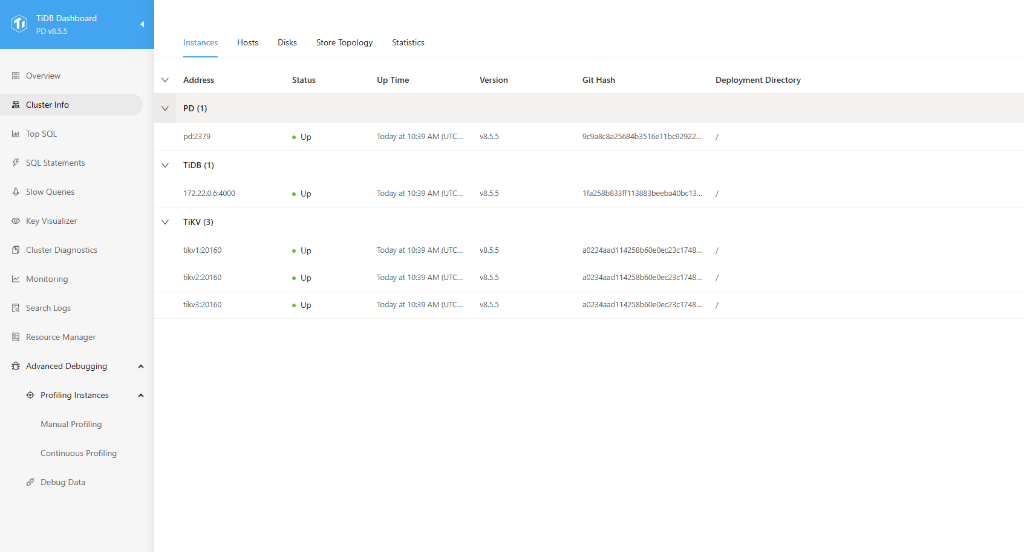
\includegraphics[width=0.92\textwidth]{figures/tidb_dashboard_topology.png}
}{
  \fbox{\parbox[c][5.5cm][c]{0.9\textwidth}{\centering
    \fontsize{12}{15}\selectfont\bfseries Minh chứng Giao diện TiDB Dashboard và Bản đồ Topology Cụm 3 Node TiKV}}
}
\caption{TiDB Dashboard (Cluster Info) trên máy M2: 1 PD, 1 TiDB Server và 3 TiKV phiên bản v8.5.5 ở trạng thái Up}
\label{fig:tidb_dashboard_topology}
\end{figure}

\begin{figure}[H]
\centering
\IfFileExists{figures/tidb_key_visualizer.png}{
  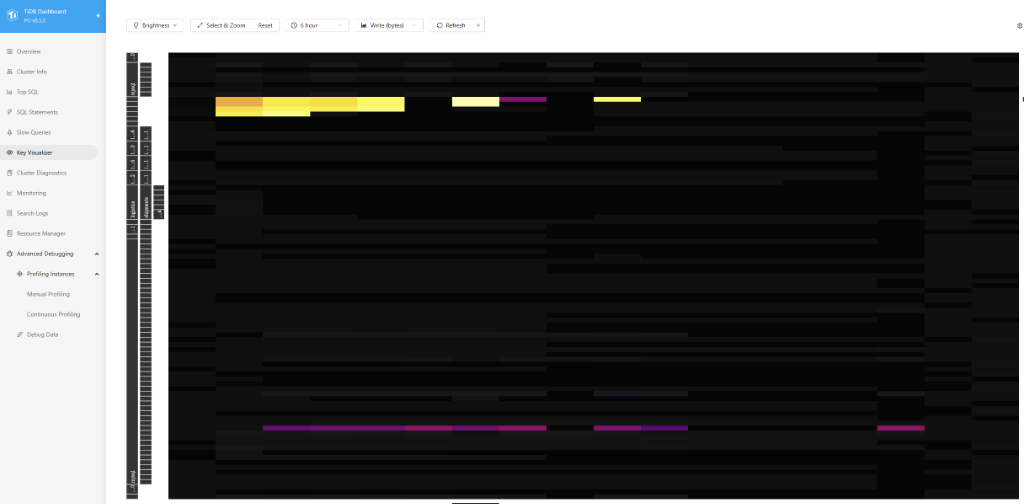
\includegraphics[width=0.92\textwidth]{figures/tidb_key_visualizer.png}
}{
  \fbox{\parbox[c][5.5cm][c]{0.9\textwidth}{\centering Key Visualizer}}
}
\caption{Key Visualizer trên máy M2, lượng byte ghi trong 6 giờ theo dải khóa}
\label{fig:tidb_key_visualizer}
\end{figure}

\subsection{Định nghĩa số node, số bản sao, quorum và khả năng chịu lỗi}
\label{sec:dinh_nghia_replica}

Số node TiKV và số bản sao của mỗi Region là hai đại lượng khác nhau. Cả hai cấu hình TiDB trong nghiên cứu đều chạy trên đúng \textbf{3 node TiKV}. Nhóm chỉ thay đổi số bản sao bằng tham số \code{replication.max-replicas} của PD, và chỉ bắt đầu đo sau khi mọi Region có đủ số peer, không còn peer chờ hoặc hỏng.

\begin{table}[H]
\centering
\caption{Định nghĩa cấu hình bản sao và khả năng chịu lỗi}
\label{tab:dinh_nghia_replica}
\bangfont
\begin{tabularx}{\linewidth}{@{}>{\raggedright\arraybackslash}p{3.0cm}YYY@{}}
\toprule
\textbf{Thuộc tính} & \textbf{TiDB RF=3} & \textbf{TiDB RF=1} & \textbf{MySQL}\\
\midrule
Node lưu trữ & 3 TiKV & 3 TiKV & 1 node\\
Bản sao mỗi Region & 3 (1 Leader, 2 Follower) & 1 & Không áp dụng\\
Quorum khi ghi & 2/3 & 1/1 & Không áp dụng\\
Khi mất 1 TiKV & Region còn 2/3 bản sao, bầu lại Leader rồi phục vụ tiếp & Region trên node đó không truy cập được & Mất node thì ngừng phục vụ\\
Khi mất 2 TiKV & Region có 2 peer trên các node đó mất quorum & Chỉ còn các Region trên node sống & Không áp dụng\\
PD / TiDB Server & 1 / 1, là điểm lỗi đơn & 1 / 1, là điểm lỗi đơn & Không áp dụng\\
\bottomrule
\end{tabularx}
\end{table}

Một node TiKV không thể tạo thành thiết lập 3 bản sao hợp lệ, vì các peer của cùng một Region phải nằm trên các store khác nhau. Ba TiKV trong thực nghiệm là ba container dùng chung một máy và một ổ đĩa. Vì vậy RF=3 ở đây chỉ chịu được lỗi ở mức tiến trình hoặc container, không chịu được lỗi của máy vật lý.
